\documentclass[12pt, a4paper]{article}
\usepackage{geometry}
\usepackage{multicol}
\usepackage{multirow}
\usepackage[table]{xcolor}
\usepackage{enumerate}
\usepackage{listings}
\usepackage{minted}
\geometry{margin=1in}

\usepackage[utf8]{inputenc}
\usepackage[T1]{fontenc}
\usepackage{graphicx}
\usepackage{ragged2e}

\usepackage{minted}
\usepackage{rotating}
\usepackage{hyperref}
\usepackage{float}
\usepackage{pstricks}
\usepackage{makecell}
\usepackage{fancyhdr}
\pagestyle{fancy}
\fancyhead{}
\fancyfoot{}

\fancyhead[l]{Laboratorio de Computación Gráfica e Interacción humano-computadora}
\fancyhead[r]{Grupo: 02}
\fancyfoot[r]{\thepage}

\usepackage{amsmath}
\usepackage{tikz}
\usepackage{longtable}
\usetikzlibrary{automata, positioning, arrows,shapes.misc, shapes.arrows, chains,matrix,positioning,% wg. " of "
	scopes,%
	decorations.pathmorphing,% /pgf/decoration/random steps | erste Graphik
	shadows}
\renewcommand{\refname}{Referencias}
\renewcommand{\contentsname}{Contenidos}
\renewcommand{\figurename}{Figura}
\renewcommand{\partname}{Parte}

\begin{document}
	
	\begin{titlepage}
		
		\newcommand{\HRule}{\rule{\linewidth}{0.5mm}} % Define comando para lineas horizontales
		
		\centering % Centra todo en la pagina
		
			%----------------------------------------------------------------------------------------
		%   LOGO SECTION
		%----------------------------------------------------------------------------------------
		
		
\includegraphics[scale = 0.235]{img/logo.png} % Logo
		\hspace{4cm}
		
\includegraphics[scale = .32]{img/fi.png}\\[.65cm] % Logo
	%----------------------------------------------------------------------------------------
		%   ENCABEZADO
		%----------------------------------------------------------------------------------------
		
		\textsc{\large \bfseries UNIVERSIDAD NACIONAL AUTÓNOMA DE MÉXICO}\\[.5cm] % Nombre de universidad
		\textsc{\large FACULTAD DE INGENIERÍA}\\[0.5cm] % Division
		\textsc{\large Ingeniería en Computación}\\[1.4 cm] % Carrera
		
		%----------------------------------------------------------------------------------------
		%   TITLE SECTION
		%----------------------------------------------------------------------------------------
		{\large LABORATORIO DE COMPUTACIÓN GRÁFICA\\ E INTERACCIÓN HUMANO COMPUTADORA}\\[.4 cm] % Materia
		% llllllllllllllllllllllllllllllllllllll
		\textsc{\large Grupo: 02}\\[1.5 cm]
		\textsc{\large Práctica Número 7}\\[1.0 cm]
		{\large Alumna: Pamela Salgado Fernández Pamela}\\[.3 cm]
		{\large Número de Cuenta: 313236505}\\[.3 cm]
		{\large Email: pame501@yahoo.com.mx}\\[1.6 cm]
		\raggedleft 
		{\large Semestre 2019-2}\\[.3 cm]
		\textsc{\large Grupo de teoría: 1}\\[.3 cm]
		{\large Fecha de entrega límite: 25/03/2019}\\[.5 cm].

			%----------------------------------------------------------------------------------------
		
		\vfill % Llenar el resto de la página con espacio en blanco
		 
		
	\end{titlepage}
	\tableofcontents
	\newpage
	\noindent
\section{Desarrollo de la práctica}
\justify

Para el ejercicio en casa, el profesor nos pidió algo similar al ejercicio realizado en clase, solo que ahora la figura a realizar, fue un dodecaedro y no un cuboy para ello también fue necesario utilizar otra imagen para realizar el texturizado.\\[0.1cm]

\justify
\subsection{Creación del dodecaedro}
\vspace{.4cm}
\justify
Para el dodecaedro se utilizó Geogebra, de esta forma fue mucho más fácil obtener las coordenadas de cada uno de los vértices y también de dibujar la figura. \\[0.2cm]
\justify
\centering 
		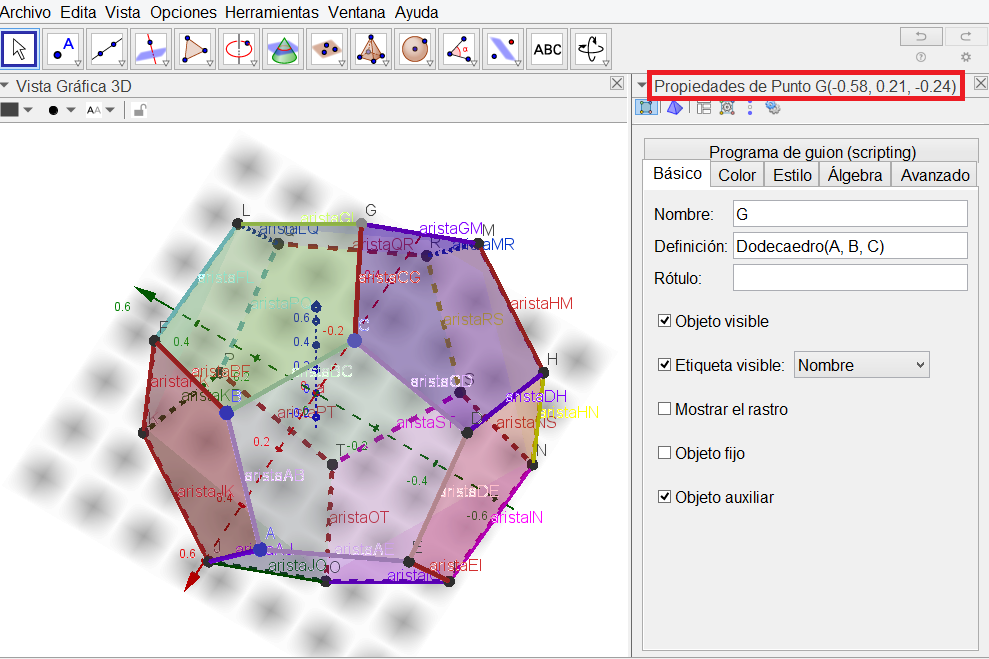
\includegraphics[scale = .44]{img/dod1.png}\\[.05cm] % Imagen1
		Figura 1: Dibujo en geogebra\\[.65cm]

 \raggedright 	
\justify
Una vez obtenidos los puntos, estos vértices se agregaron al código, junto con sus indices correspondientes, a continuación se muestra un pequeño fragmento del código :
\begin{minted}[breaklines]{C++}
//***********************************************************

GLfloat cubo_vertices[] = {
	//x      y       z      u	   v
	0.3f,  0.0f,  -0.6f,   0.18f, 0.36f,   //0   A
	0.11f, -0.38f, -0.6,  0.15f,  0.6f,   //1    E
	-.31f, -0.31f, -0.6f,  .04f, 0.6f,   //2    D
	-0.38f, 0.11f, -0.6f,  0.01f,0.36f,   //3	c
	0.0f,  0.3f,  -0.6f,  0.1f,	 0.24f,   //4    B
	//--------------------------------------
	0.03f,  0.52f,  -0.24f,   0.31f, 0.36f,   //5   F
	0.36f,  0.36f,  -0.02f,   0.36f, 0.62f,   //6   K
	0.52f,  0.03f,  -0.24f,   0.26f, 0.76f,   //7   J

	-0.38f, 0.11f, -0.6f,  0.16f,0.16f,   //8	C
	0.0f,  0.3f,  -0.6f,  0.2f,  0.36f,   //9   B
	-0.32f, 0.46f, -0.02f,  0.36f,0.16f,   //10	L
	-0.58f,  0.21f,  -0.24f,  0.26f,  0.02f,   //11  G
	//CARA MORADA 2
	0.3f,  0.0f,  -0.6f,   0.16f, 0.6f,     //12   A
	0.11f, -0.38f, -0.6,  0.06f,  0.76f,      //13   E
	0.52f,  0.03f,  -0.24f,   0.26f, 0.76f,  //14   J
	0.21f,  -0.58f,  -0.24f,  0.1f,  0.9f,   //15   I
	0.46f, -0.32f,   -0.02f,  0.22f, 0.9f,   //16	O
	//CARA VERDE FUERTE 5
	0.52f,  0.03f,  -0.24f,   0.26f, 0.76f,  //17   J
	0.46f, -0.32f,   -0.02f,  0.3f, 0.9f,   //18	O
	0.36f,  0.36f,  -0.02f,   0.36f, 0.6f,  //19   K
	0.27f, -0.22f,   0.34f,   0.41f, 0.9f,   //20	T
	0.2f,    0.2f,  0.34f,   0.45f, 0.76f,  //21   P
	//CARA AZUL 6
	0.03f,  0.52f,  -0.24f,   0.31f, 0.36f,  //22   F
	0.36f,  0.36f,  -0.02f,   0.36f, 0.6f,  //23   K
	-0.22f, 0.27f,   0.34f,   0.52f, 0.36f,   //24	Q
	0.2f,    0.2f,  0.34f,   0.48f, 0.6f,  //25   P
	-0.32f, 0.46f, -0.02f,  0.42f,0.22f,   //26	L

	//CARA VERDE, DIVISION 7
	-0.22f, 0.27f,   0.34f,   0.52f, 0.36f,   //27	Q
	0.2f,    0.2f,  0.34f,   0.48f, 0.6f,  //28   P
	0.27f, -0.22f,   0.34f,   0.58f, 0.76f,   //29	T
	-0.41f, -0.11f,  0.34f,   0.63f, 0.36f,  //30   R
	-0.11f, -0.41f,   0.34f,   0.68f, 0.6f,   //31	S

	//CARA AZUL FUERTE 8
	-0.32f, 0.46f, -0.02f,  0.595f,0.02f,   //32	L
	-0.22f, 0.27f,   0.34f,   0.55f, 0.22f,   //33	Q
	-0.41f, -0.11f,  0.34f,   0.64f, 0.36f,  //34  R
	-0.63f, -0.15f,  -0.02f,   0.75f, 0.22f,   //35	M
	-0.58f,  0.21f,  -0.24f,  0.705f,  0.02f,   //36  G
	
	//cara rosa
	-0.11f, -0.41f,   0.34f,   0.68f, 0.6f,   //37	S
	0.27f, -0.22f,   0.34f,   0.645f, 0.84f,   //38	T
	0.46f, -0.32f,   -0.02f,  0.73f, 0.9f,   //39	O
	0.21f,  -0.58f,  -0.24f,  0.83f,  0.84f,   //40   I
	-0.15f,  -0.63f,  -0.02f,  0.8f,  0.6f,   //41   N

//***********************************************************	
	INDICES
//***********************************************************	

void CrearCubo(){
	unsigned int cubo_indices[] = {
		// CARA 1
		0, 1, 2,
		3,2,0,
		0,3,4,

		58,57,61,
		57,60,61,
		60,57,59,

		9,8,5,
		8,11,5,
		5,10,11,

		12,13,15,
		15,12,16,
		16,14,12,

		18,14,20,
		20,14,19,
		19,21,20,
		
		//CARA AZUL CLARO 
		23,22,25,
		25,22,24,
		24,22,26,
		
		//CARA VERDE 
		27,28,29,
		29,27,31,
		30,31,27,
		
		//cara azul
		32,33,36,
		36,35,33,
		33,34,35,
		//cara rosa
		37,41,40,
		40,39,37,
		37,38,39,
	
	};
\end{minted}
\vspace{.1cm}
Este mismo proceso se realizó para cada uno de los vértices, y como se puede observar en el código, también fue necesario añadir las coordenadas de la imagen que utilizaríamos para texturizar. 
\subsection{Imagen para texturizado}
\vspace{.5cm}
\justify
\centering 
		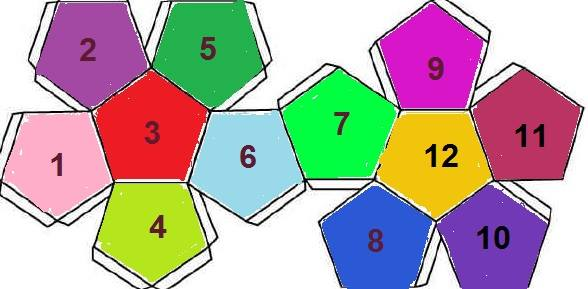
\includegraphics[scale = .54]{img/dod.jpg}\\[.05cm] % Imagen1
		Figura 2: Imagen\\[.65cm]

 \raggedright 	
\justify

\subsection{Código}
Anexo a este documento, se encuentran los programas utilizados para esta práctica.\\[.1cm]	
\subsection{Ejecución del programa}	
\centering 
		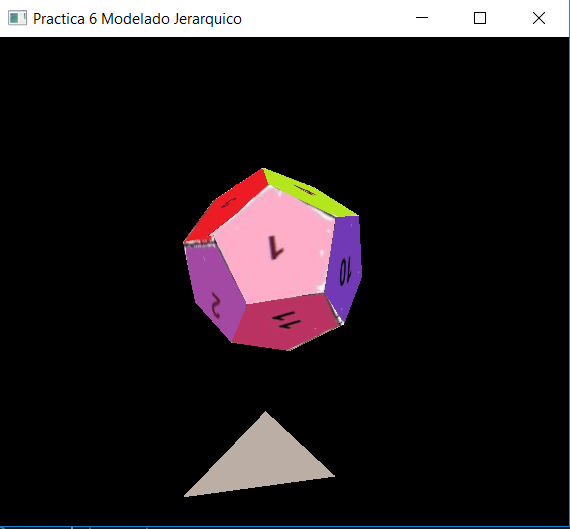
\includegraphics[scale = .89]{img/ej1.png}\\[.05cm] % Imagen1
		Figura 3: Rotación sólo de estrellas\\[.65cm]
		
		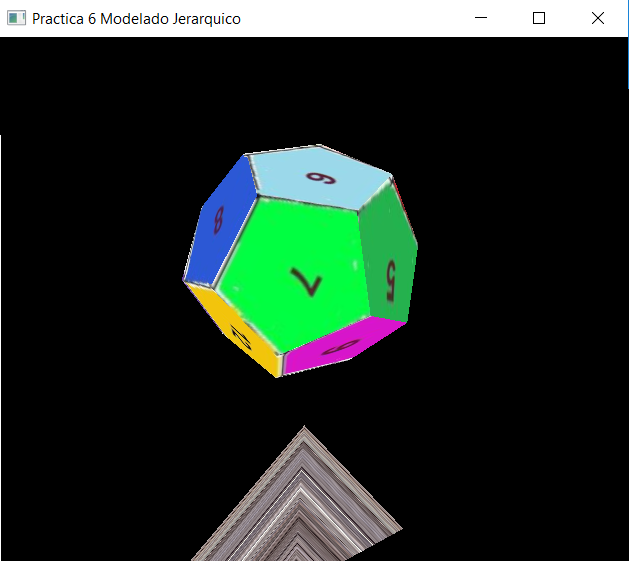
\includegraphics[scale = .84]{img/ej2.png}\\[.05cm] % Imagen1
		Figura 4: Rotación de todos los elementos\\[.65cm]

 \raggedright 	
\section{Problemas presentados}
\justify
No se presentaron problemas al realizar esta práctica. \\[.4cm]

\section{Comentarios}
\justify
El uso de Geogebra facilitó demasiado la realización de este ejercicio, además aprendí que a utilizar el archivo stb image, el cual nos permite cargar imágenes, ya que lo que necesitamos es que OpenGL pueda leer una imagen, nos permite obtener información de una imagen para posteriormente almacenarla en un arreglo de datos y ese arreglo de datos pasárselo a OpenGL.\\[.3cm]
Así mismo, tambien comprendí que es la textura, ahora se que es un arreglo de datos, ya sea en 2d, 3d o una textura basada en un fractal, y contiene información de color, ilumiación y normales.\\[.3cm]
Fue una práctica muy interesante ya que vimos varios conceptos nuevos, utilizamos más librerías y logramos observar como es posible texturizar con pocas lineas de código.

\end{document}